\documentclass[14pt,a4paper]{scrartcl}
\usepackage{cmap}
\usepackage[utf8]{inputenc}
\usepackage[T1,T2A]{fontenc}
\usepackage[english,russian]{babel}
\usepackage{relsize}
\usepackage{graphicx}
\usepackage{subfigure}
\usepackage{mathtools}
\usepackage{amssymb}
\usepackage{float}
\usepackage{sidecap}
\usepackage{wrapfig}
\usepackage{caption}
\usepackage[table,xcdraw]{xcolor}
\usepackage{listings}
\begin{document}
	\begin{titlepage}
	\begin{center}
		\large
		МИНИСТЕРСТВО ОБРАЗОВАНИЯ И НАУКИ\\ РОССИЙСКОЙ ФЕДЕРАЦИИ
		
		\vspace{0.5cm}
		
		МГТУ им Н.Э.Баумана
		\vspace{0.25cm}
		
		Факультет ФН
		
		Кафедра вычислительной математики и математической физики
		\vfill
		
		
		Соколов Арсений Андреевич\\
		\vfill
		
		
		{\LARGE Домашнее задание №1 по математической статистике\\[2mm]
		}
		\bigskip
		
		3 курс, группа ФН11-53Б\\
		Вариант 9
	\end{center}
	\vfill
	
	\newlength{\ML}
	\settowidth{\ML}{«\underline{\hspace{0.7cm}}» \underline{\hspace{2cm}}}
	\hfill\begin{minipage}{0.4\textwidth}
		Преподаватель\\
		\underline{\hspace{3cm}} Т.\,В.~Облакова\\
		«\underline{\hspace{0.7cm}}» \underline{\hspace{1.71cm}} 2019 г.
	\end{minipage}%
	\bigskip
	
	
	\vfill
	
	\begin{center}
		Москва, 2019 г.
	\end{center}
\end{titlepage}

\section{Подготовка данных}
\subsection{Поиск крайних элементов вариационного ряда}
Импортируем данные, сохранённые в формате $.csv$, определяем максимальный, минимальный.


\begin{lstlisting}
	> df <- read.csv("db.csv", header = F) #data import
	> max_el <- max(df)
	> max_el
	[1] 17.985
	> min_el <- min(df)
	> min_el
	[1] 2.375
	> range_el <- max_el - min_el
	> range_el
	[1] 15.61
\end{lstlisting}
\subsection{Вариационный ряд}
Выведем на печать упорядоченную выбору -- вариационный ряд:
\begin{lstlisting}
> sort(df$V1)
	[1]  2.375  2.666  2.744  2.867  2.903  3.086  3.375
	[8]  3.377  3.608  3.635  3.878  4.354  4.646  4.715
	[15]  4.727  4.843  4.942  4.964  5.006  5.140  5.175
	[22]  5.333  5.343  5.647  5.743  5.811  5.814  6.078
	[29]  6.339  6.355  6.542  6.734  6.875  6.883  7.039
	[36]  7.175  7.241  7.357  7.479  7.683  8.206  8.250
	[43]  8.282  8.415  8.428  8.592  8.681  8.905  8.916
	[50]  9.012  9.097  9.159  9.182  9.234  9.354  9.458
	[57]  9.493  9.838  9.861  9.869  9.919  9.927 10.268
	[64] 10.351 10.511 10.821 11.093 11.095 11.449 12.040
	[71] 12.173 12.175 12.177 12.423 12.622 12.767 12.768
	[78] 12.888 12.906 12.911 12.924 12.959 12.959 13.325
	[85] 13.480 13.535 13.890 13.924 13.957 14.022 14.186
	[92] 14.237 14.286 14.396 14.495 14.612 14.919 15.134
	[99] 15.238 15.308 15.439 15.506 15.535 15.649 15.694
	[106] 15.850 15.864 15.988 15.992 16.058 16.175 16.195
	[113] 16.892 17.103 17.117 17.690 17.757 17.921 17.963
	[120] 17.985
\end{lstlisting}

\section{Построение гистограммы частот}
\subsection{Определение количества интервалов разбиения}
Определим число "столбиков" гистограммы определим по правилу Стёрджеса:
\begin{equation*}
	n = 1 + [\log_2{N}],
\end{equation*}
где $N$ -- общее число наблюдений.


\begin{lstlisting}
	> num_bins = round(1 + log2(length(df$V1)))
	> num_bins
	[1] 8
\end{lstlisting}

\subsection{Определение ширины интервала}
Определим ширину интервала группировки оп формуле:
\begin{equation*}
	\text{width} = \frac{\text{range}}{n},
\end{equation*}
где $\text{range}$ -- размах выборки.


\begin{lstlisting}
	> bin_width <- range_el / num_bins
	> bin_width
	[1] 1.95125
\end{lstlisting}


\subsection{Построение графика}
По полученным данным построим гистограмму частот:


\begin{lstlisting}
	> png(filename = "../img/hist_without_dens.png", 
	+     width = 1920, height = 1080,
	+     pointsize = 24, res = 96 * 1.25)
	> par(mar = c(3, 3, 2, 1), xaxs = "i", yaxs = "i")
	> pl1 <- hist(df$V1,
	+        breaks = seq(min_el, max_el, by = bin_width), 
	+        xlim = c(0, 20), ylim = c(0.00,0.10), 
	+				axes = F, freq = F,
	+        main = "Histogram of data")
	> axis(1, seq(0, 20, 1))
	> axis(2, seq(0.00, 0.10, 0.01), las = 1)
	> grid(nx = 20, ny = 10, equilogs = F)
	> dev.off()
	RStudioGD 
	2 
\end{lstlisting}

\begin{figure}[t!]
	\center{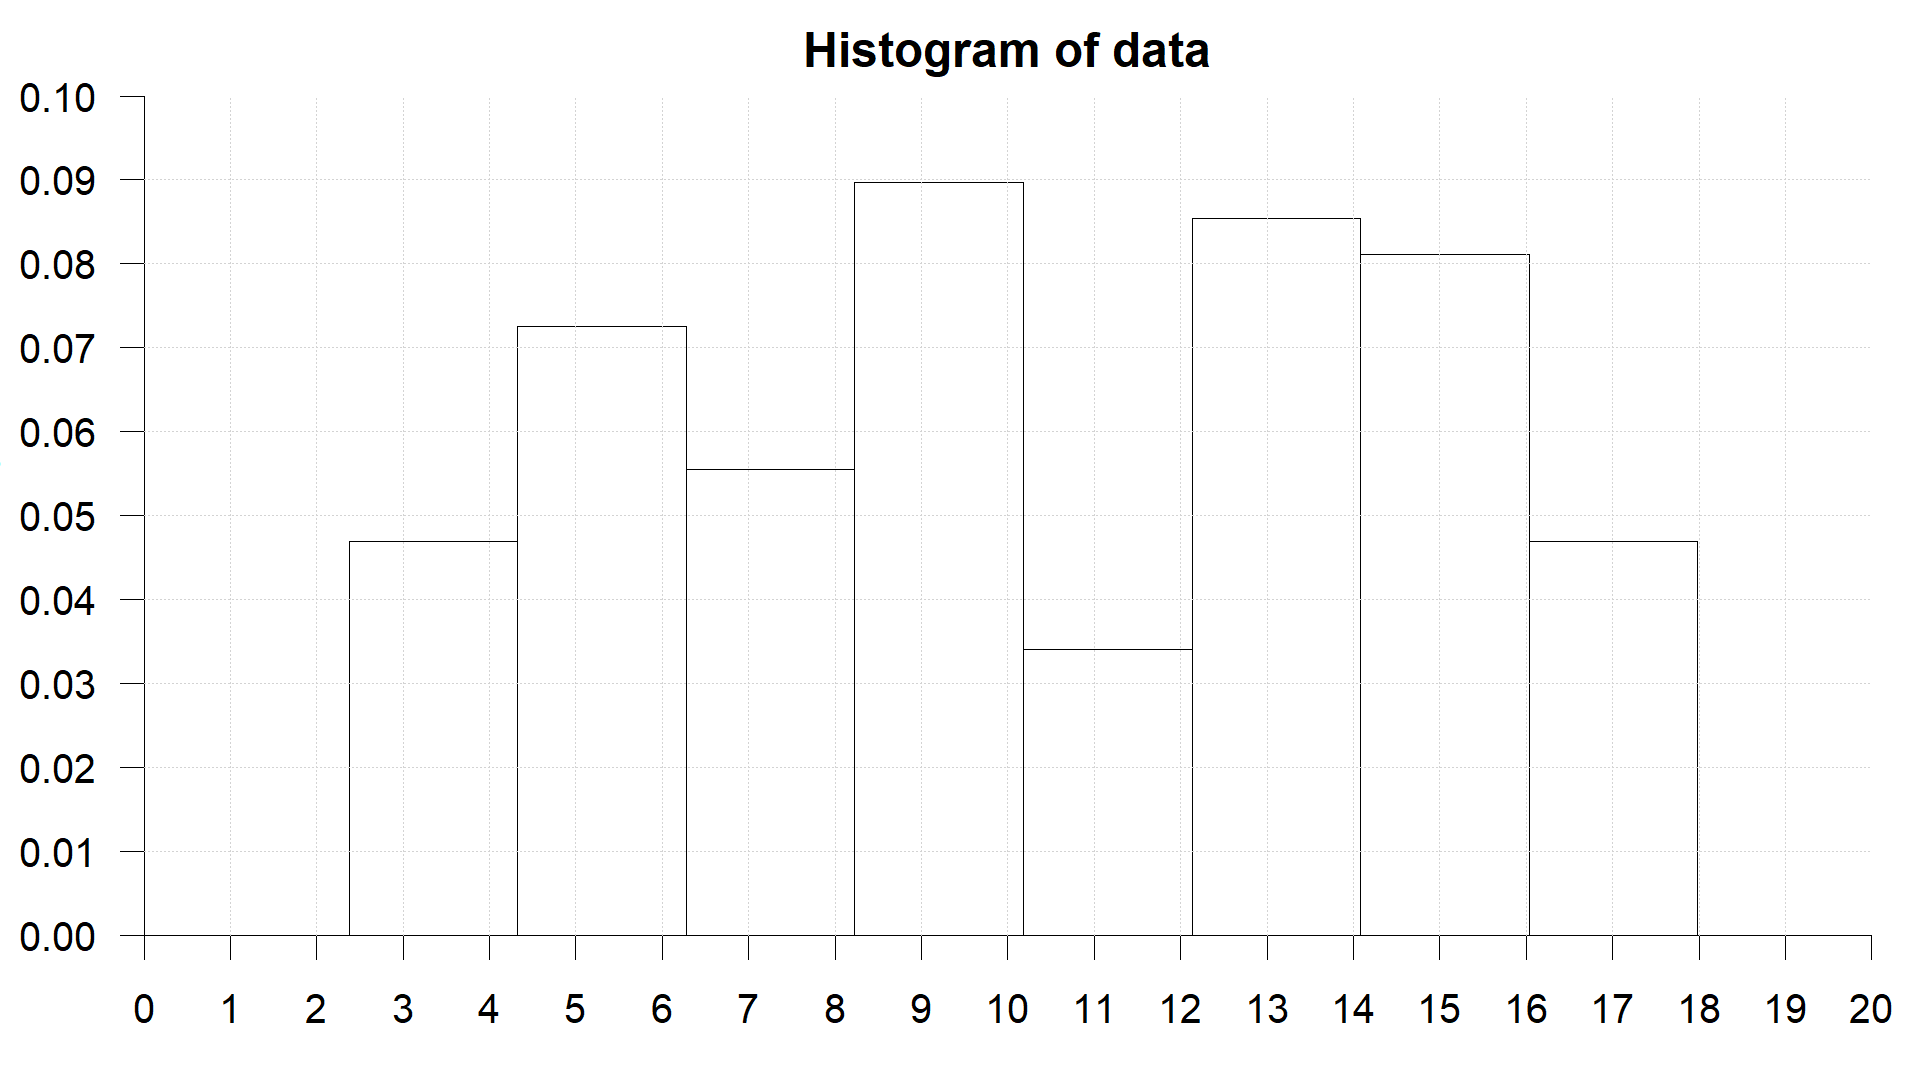
\includegraphics[width=1\linewidth]{../img/hist_without_dens.png}}
	\caption{Гистограмма частот выборки.}
	\label{ris:hist_without_dens}
\end{figure}

\subsection{Определение относительных частот}
Для начала определим количество элементов в каждом интервале:
\begin{lstlisting}
	> pl1$counts
	[1] 11 17 13 21  8 20 19 11
\end{lstlisting}

Посчитаем относительную частоту (эмпирическую вероятность) для каждого интервала:
\begin{lstlisting}
	> relative_freq <- pl1$counts / length(df$V1)
	> relative_freq
	[1] 0.09166667 0.14166667 0.10833333 0.17500000
	[5] 0.06666667 0.16666667 0.15833333 0.09166667
\end{lstlisting}

\subsection{Меры центральной тенденции}
Определим выборочные среднее и медиану (мода в нашей выборке будет неинформативной):
\begin{lstlisting}
	> mean_el <- mean(df$V1)
	> mean_el
	[1] 10.2681
	> median_el <- median(df$V1)
	> median_el
	[1] 9.894
\end{lstlisting}

\subsection{Меры изменчивости}
Определим размах(определялся ранее), дисперсию и стандартное отклонение:
\begin{lstlisting}
	> range_el
	[1] 15.61
	> var_el <- var(df$V1)
	> var_el
	[1] 19.61091
	> sd_el <- sd(df$V1)
	> sd_el
	[1] 4.42842
\end{lstlisting}


\section{Определение возможного закона распределения}
Анализ возможного закона распределения начнём с построения Cullen and Frey skewness-kurtosis графика, предварительно запустрэпив $10^4$ ресэмплов:
\begin{lstlisting}
	> png(filename = "../img/cullen_and_frey_graph.png", 
	+     width = 1920, height = 1080,
	+     pointsize = 24, res = 96 * 1.25)
	> descdist(df$V1,method = "sample", boot = 1e4)
	summary statistics
	------
	min:  2.375   max:  17.985 
	median:  9.894 
	mean:  10.2681 
	sample sd:  4.40993 
	sample skewness:  -0.02444883 
	sample kurtosis:  1.822814 
	> dev.off()
	RStudioGD 
	2 
\end{lstlisting}

Где $\text{kurtosis} = \frac{\mu_4}{\sigma^4} - 3$ -- это коэффициент эксцесса, а $\text{skewness} = \frac{\mu_3}{\sigma^3} $ -- коэффициент асимметрии.

\begin{figure}[t!]
	\center{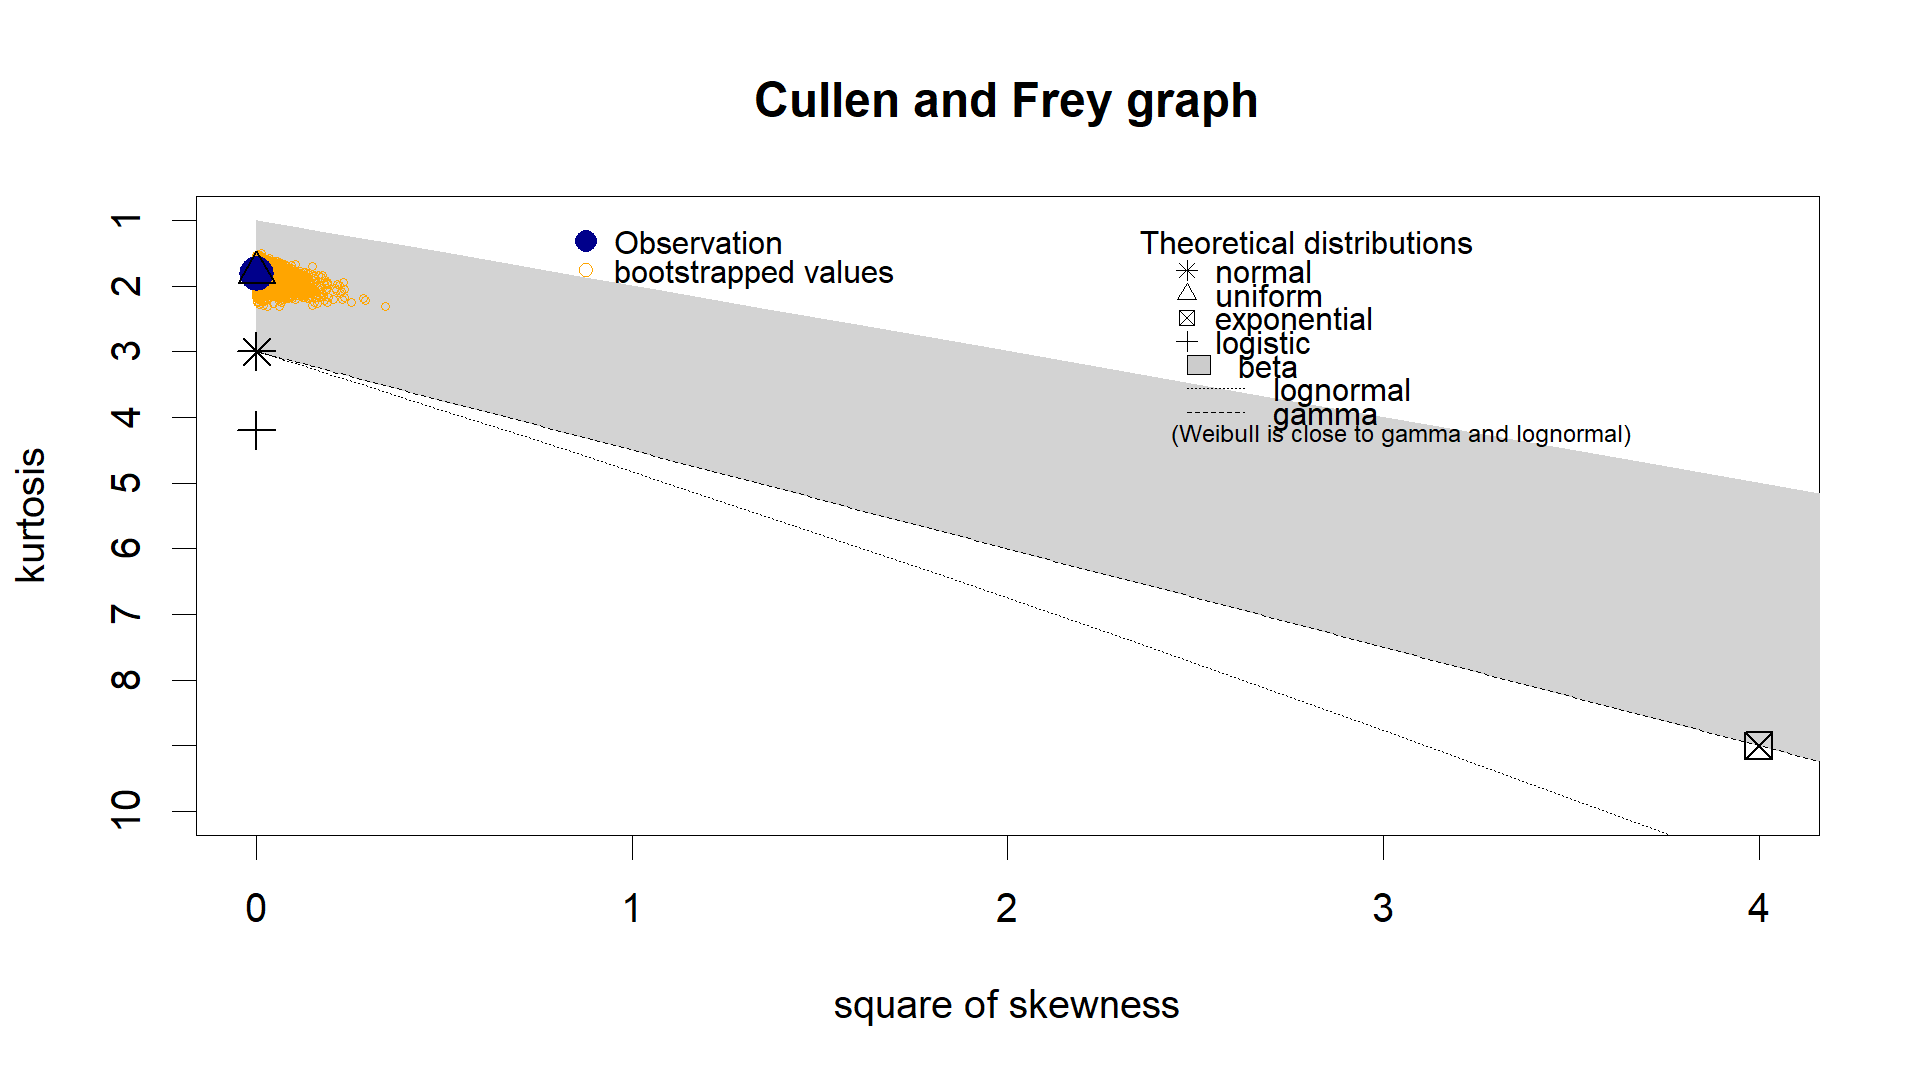
\includegraphics[width=1\linewidth]{../img/cullen_and_frey_graph.png}}
	\caption{Cullen and Frey skewness-kurtosis plot.}
	\label{ris:cullen_and_frey_graph}
\end{figure}

\pagebreak
Из Рис.~\ref{ris:cullen_and_frey_graph} мы видим, что наша выборка близка больше всего к $\text{uniform}$ -- равномерному распределению и $\text{beta}$ -- бета-распределению. Так же рассмотрим нормальное распределение для сравнения моделей.

Для анализа нашего датасета на принадлежность к бета-распределению, засрескейлим данные к интервалу $[0;1]$:
\begin{lstlisting}
	> library(scales)
	> res <- rescale(df$V1)
	> res
	[1] 0.77642537 0.19013453 0.77008328 0.67347854
	[5] 0.00000000 0.43939782 0.22011531 0.15067265
	[9] 0.15810378 0.06418962 0.40397181 0.62767457
	[13] 0.14990391 1.00000000 0.39827034 0.50563741
	[17] 0.99590006 0.23721973 0.31172325 0.14548366
	[21] 0.48379244 0.88532992 0.16854580 0.98539398
	[25] 0.30749520 0.87232543 0.37354260 0.43606662
	[29] 0.43062140 0.16585522 0.22030750 0.84304933
	[33] 0.86412556 0.61915439 0.07898783 0.28878924
	[37] 0.38776425 0.73766816 0.75989750 0.20960922
	[41] 0.86322870 0.25496477 0.04554773 0.48327995
	[45] 0.08071749 0.66579116 0.03151826 0.01864190
	[49] 0.55848815 0.47809097 0.31915439 0.37841127
	[53] 0.58129404 0.74196028 0.28827675 0.94439462
	[57] 0.99859065 0.02363869 0.62793081 0.47956438
	[61] 0.06406150 0.73984625 0.54106342 0.03382447
	[65] 0.55861627 0.67495195 0.09628443 0.51095452
	[69] 0.37636131 0.75663037 0.84119154 0.21575913
	[73] 0.67463165 0.42517617 0.66572710 0.87206919
	[77] 0.45598975 0.85323511 0.18949391 0.92998078
	[81] 0.17713004 0.44708520 0.34003844 0.88404869
	[85] 0.38693145 0.45374760 0.87655349 0.67802691
	[89] 0.62780269 0.76303652 0.81736067 0.64368994
	[93] 0.27924407 0.83689942 0.74612428 0.82850737
	[97] 0.41902627 0.98110186 0.67802691 0.80358744
	[101] 0.32696989 0.48007687 0.67578475 0.52120436
	[105] 0.65643818 0.78392056 0.94349776 0.29878283
	[109] 0.71140295 0.26694427 0.12677771 0.25393978
	[113] 0.71492633 0.17937220 0.43459321 0.16444587
	[117] 0.70147341 0.85035234 0.41832159 0.82402306
\end{lstlisting}

Составим наши модели, отталкиваясь от метода моментов:
\begin{lstlisting}
	> fit.norm <- fitdist(df$V1, "norm", method = "mme")
	> fit.uniform <- fitdist(df$V1, "unif", method = "mme")
	> fit.beta <- fitdist(res, "beta", method = "mme")
\end{lstlisting}

Рассмотрим критерии Колмогорова-Смирнова и Крамера-Мизеса:
\begin{lstlisting}
> stat_normal <- gofstat(fit.norm, 
+                        fitnames = c("normal"))
> stat_unif <- gofstat(fit.uniform, 
+                      fitnames = c("uniform"))
> stat_beta <- gofstat(fit.beta, 
+                      fitnames = c("beta"))
> 
> stat_table <- cbind(rbind(stat_normal$ks, stat_normal$cvm),  
+                     rbind(stat_unif$ks, stat_unif$cvm),
+                     rbind(stat_beta$ks, stat_beta$cvm))
> rownames(stat_table) <- c("Kolmogorov-Smirnov statistic", 
+                           "Cramer-von Mises statistic")
> stat_table
                               normal    uniform     beta
Kolmogorov-Smirnov statistic 0.08952502 0.04535694 0.04307507
Cramer-von Mises statistic   0.22184007 0.03095026 0.02950918
\end{lstlisting}

Отчётливо видно преобладание равномерного и бета-распределений с небольшим преимуществом у бета-распределения.

Построим несколько графиков:
\begin{lstlisting}
	> png(filename = "../img/fit_norm.png", 
	+     width = 1920, height = 1080,
	+     pointsize = 24, res = 96 * 1)
	> plot(fit.norm)
	> dev.off()
	> png(filename = "../img/fit_unif.png", 
	+     width = 1920, height = 1080,
	+     pointsize = 24, res = 96 * 1)
	> plot(fit.uniform)
	> dev.off() 
	> png(filename = "../img/fit_beta.png", 
	+     width = 1920, height = 1080,
	+     pointsize = 24, res = 96 * 1)
	> plot(fit.beta)
	> dev.off()
	RStudioGD 
	2 

\end{lstlisting}

\begin{figure}[h]
	\center{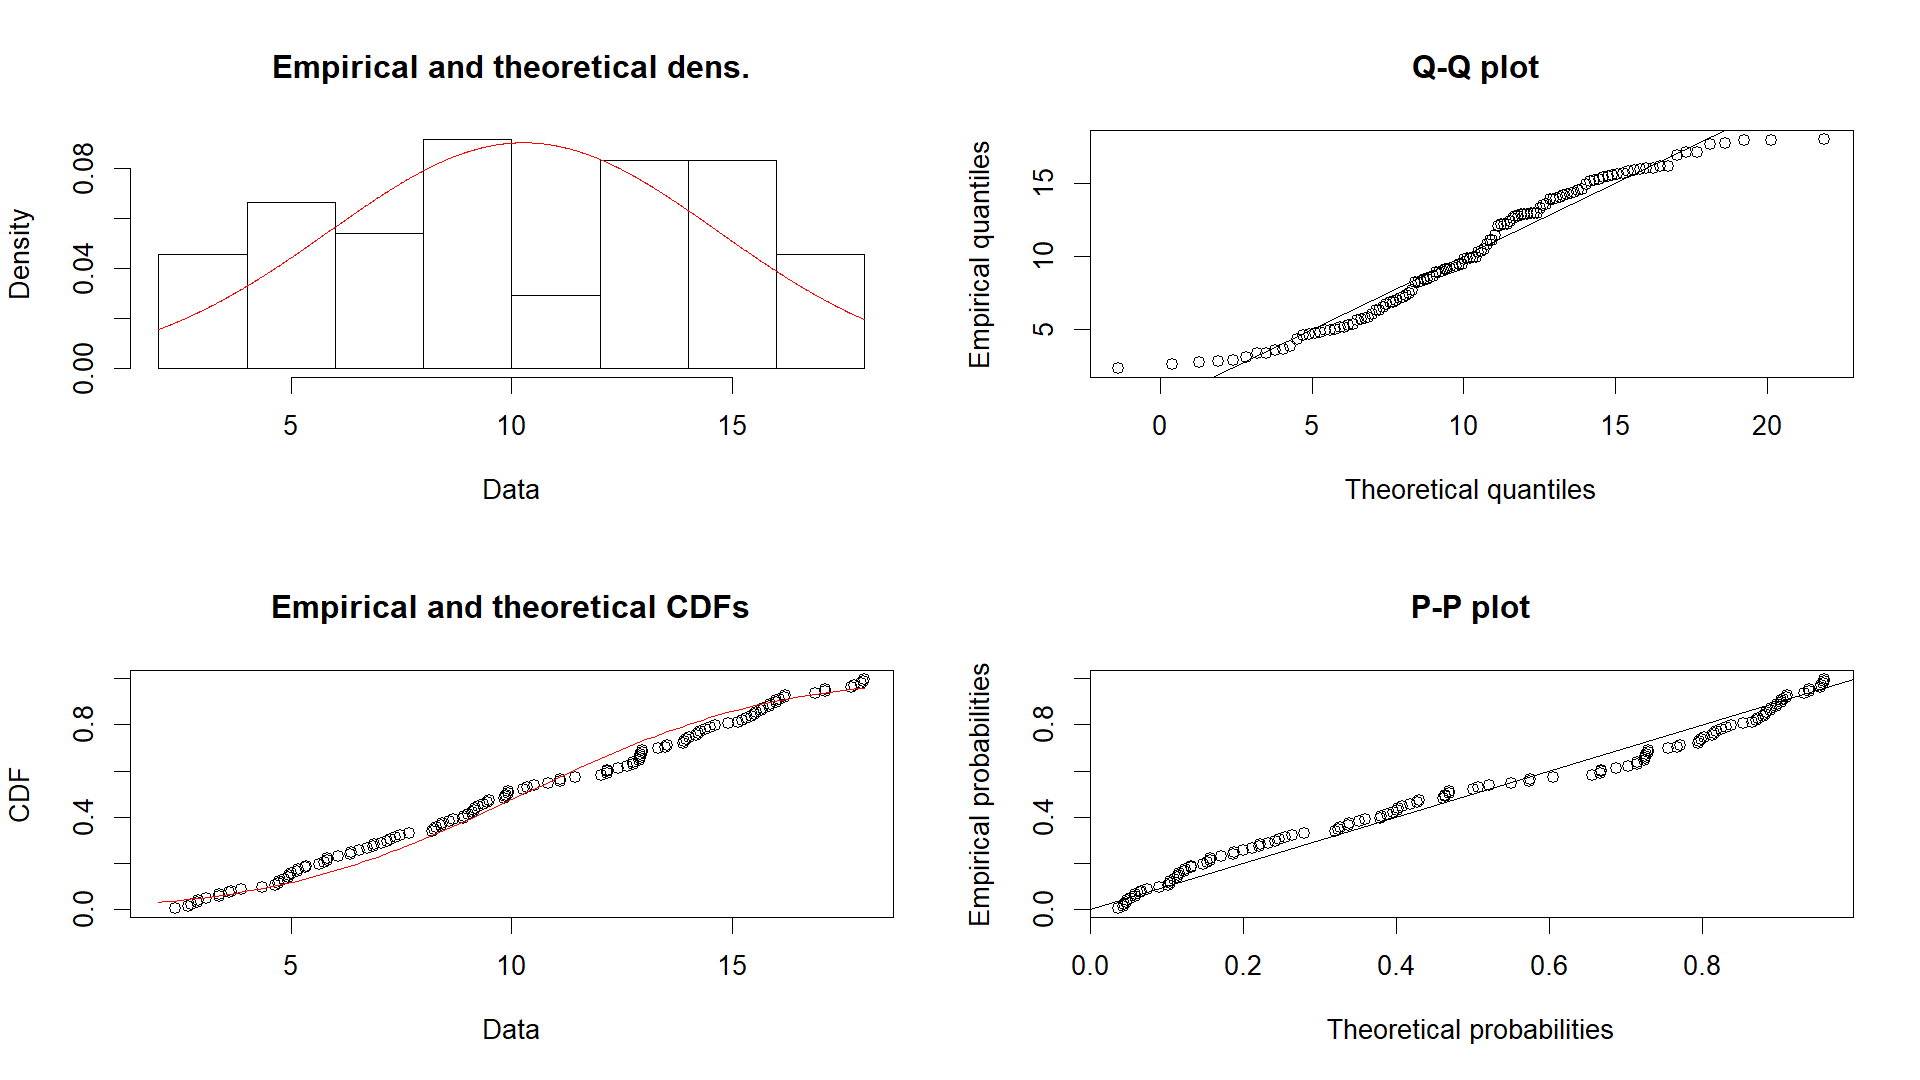
\includegraphics[width=1\linewidth]{../img/fit_norm.png}}
	\caption{Нормальное распределение.}
	\label{ris:fit_norm}
\end{figure}

\begin{figure}[b]
	\center{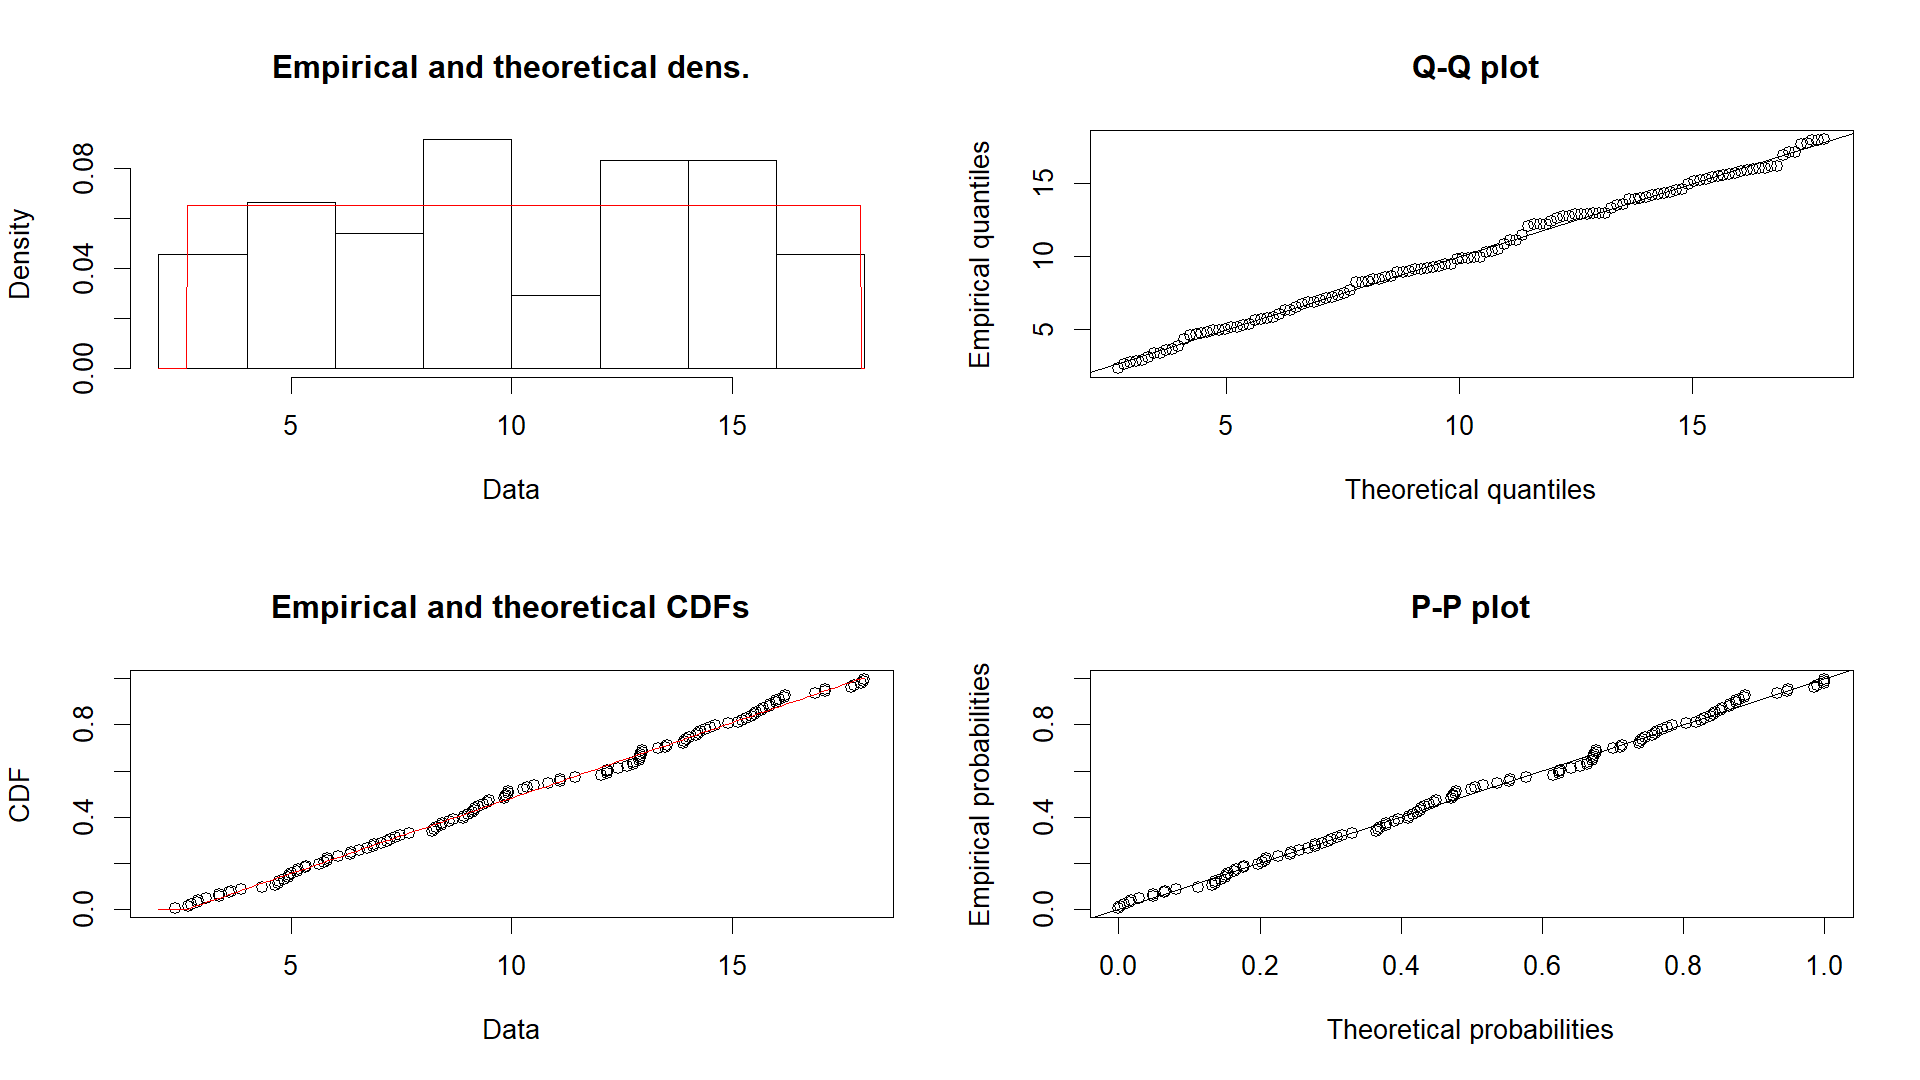
\includegraphics[width=1\linewidth]{../img/fit_unif.png}}
	\caption{Равномерное распределение.}
	\label{ris:fit_unif}
\end{figure}

\begin{figure}[b]
	\center{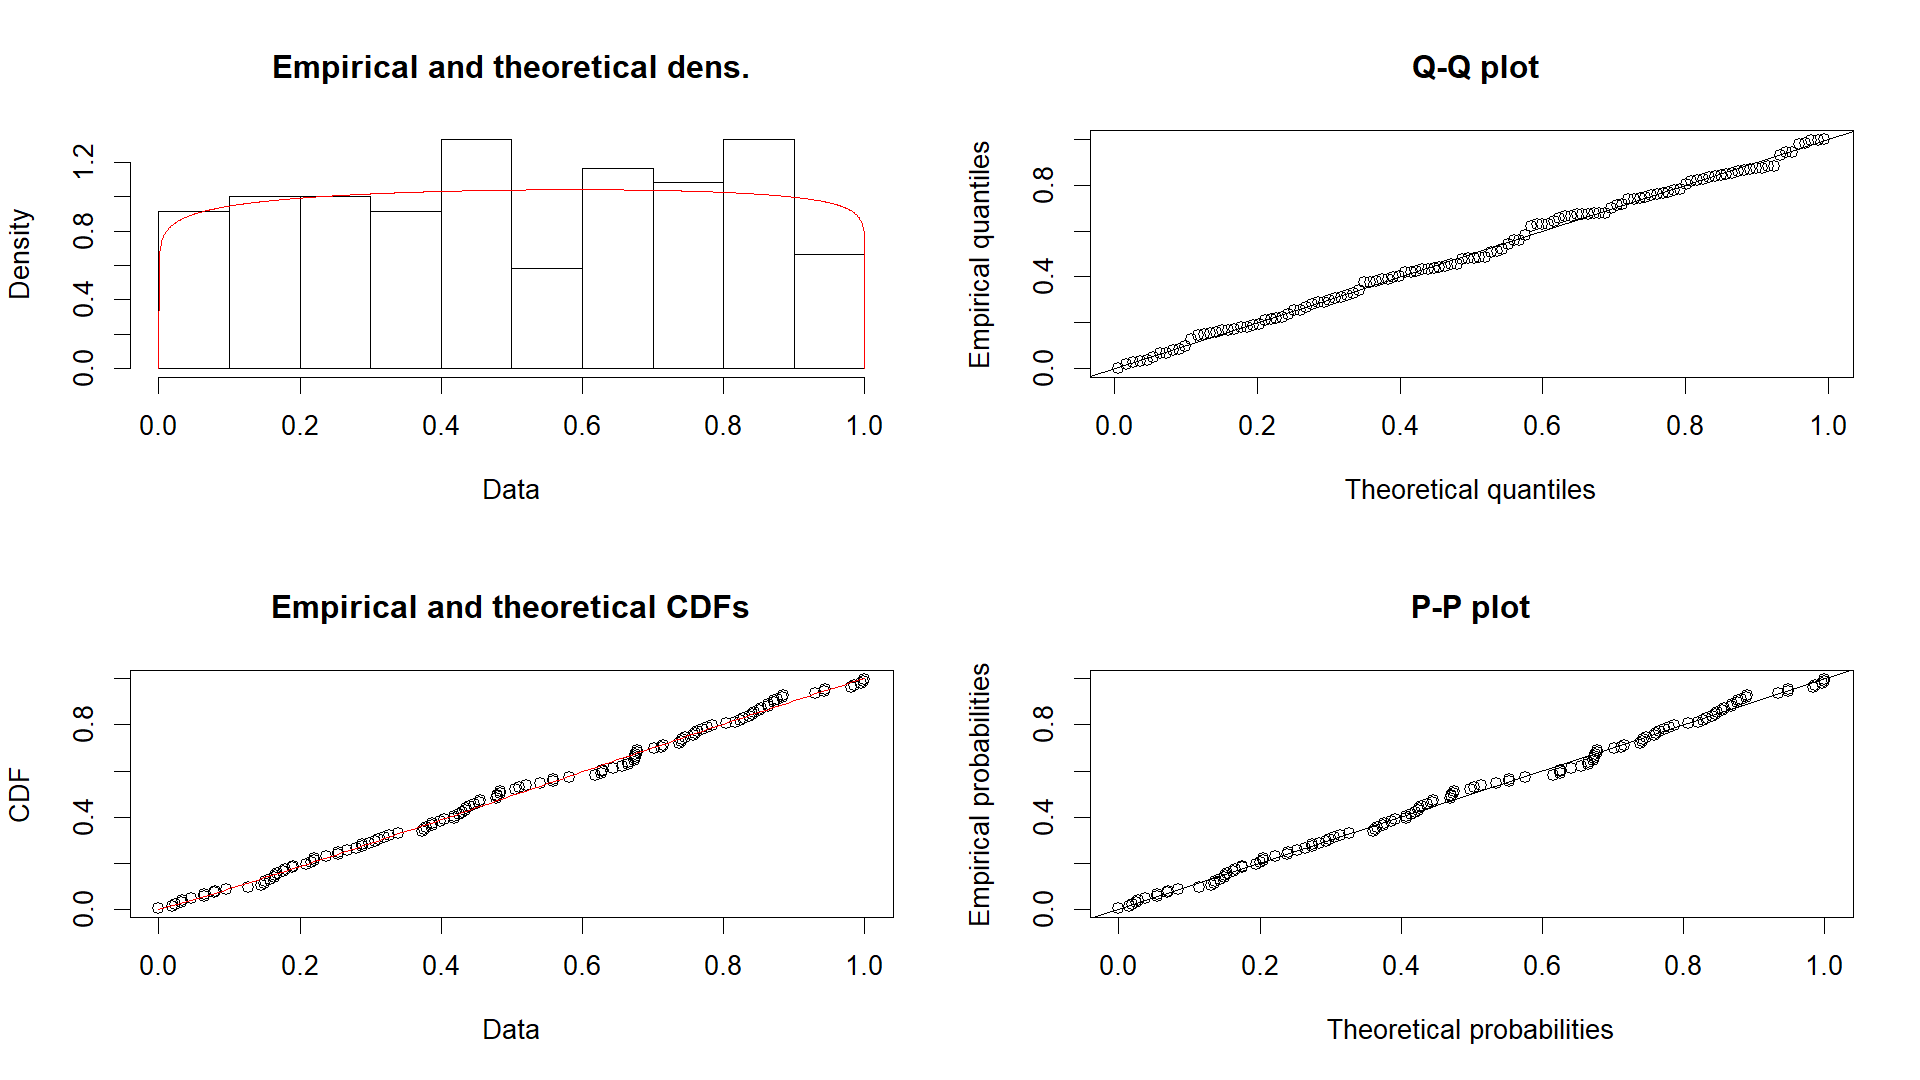
\includegraphics[width=1\linewidth]{../img/fit_beta.png}}
	\caption{Бета распределение.}
	\label{ris:fit_beta}
\end{figure}

Для простоты дальнейшего анализа рассмотрим равномерное распределение.
\pagebreak



\subsection{Оценка параметров распределения методом моментов}



\end{document}